%%%%%%%%%%%%%%%%%%%%%%%%%%%%%%%%%%%%%%%%%%%%%%%%%%%%%%%%%%%%%%%%%%%%%%%%%%%%%%%%%%%%%%%
% - BACKGROUND: BEGIN
%%%%%%%%%%%%%%%%%%%%%%%%%%%%%%%%%%%%%%%%%%%%%%%%%%%%%%%%%%%%%%%%%%%%%%%%%%%%%%%%%%%%%%%

\chapter{Background Review}
\label{ch:background}

%%%%%%%%%%%%%%%%%%%%%%%% STRUCTURED COMMUNICATIONS   %%%%%%%%%%%%%%%%%%%%%%%%%%%%%%%%%

\section{Importance of Structured Communications}
\label{sec:structuredcommms}

Communication is increasingly becoming the fundamental issue in many areas of software development, whether with respect to web applications, multi-core CPU processing, complex IT systems that communicate using standardised business protocols or sensor networks with significant amounts of processing units per square meter\cite{sessionbased_programming}.

All these examples of distributed systems inlvolve multiple remote components that independently communicate message and coordinate activities between each other. It is important that such interactions conform to an agreed structure, often referred to as a protocol, such as SMTP, POP3\cite{sess_type_guided_distr_interact} or even lower-level network protocols such as TCP and IP. These sequences of interactions as a whole form a unit of \textit{conversation}, which may involve basic message passing, repeated exchanges (i.e. loops) and branching into different communication paths\cite{sessionbased_programming}.

The study of \textit{session types} has been proposed as a type thoery for structuring the units of interaction in the context of process calculi as a way of capturing precise interaction between peers\cite{sessionbased_programming, sess_type_guided_distr_interact}. However, the \textit{session type theory} is focused on binary (two-party) interactions and does not capture the communications structures of multiparty distributed systems. The \textit{session type theory} has been extended recently in \cite{multiparty_sess_types} to cater for this more general situation. Both theories will be discussed in detail respectively in \autoref{sec:binsessiontypes} and \ref{sec:mpsessiontypes}.




%%%%%%%%%%%%%%%%%%%%%%%%%%%%%%   PI-CALCULUS    %%%%%%%%%%%%%%%%%%%%%%%%%%%%%%%%%%%%%%

\section{Pi-calculus: The Roots of Session Types}
\label{sec:picalculus}
	
As briefly discussed in \autoref{sec:intro} $\pi$-calculus is an important foundation of Session-Based Programming as it allows to understand the behaviour of communicating systems. It is an extension of the theory of sequential algorithmic processes to systems where interaction plays a significant role, which was limited by the inability of modelling physical and virtual mobility of such systems. $\pi$-calculus lets us model this effectively describing concurrent communicating processes and their interactional behaviours rigorously.

\subsection{Automaton - Basic Unit in $\pi$-calculus}
The basic unit in the model is an \textit{automaton}. Links between automata may evolve over time as automata may for example be created, split or die. They can be loosely compared to method calls in programming, i.e. when a code section is entered an automaton is created, when it executes it can make calls to other sections of code, hence creating other automata and when the code block is left, automata die.

This behaviour was already described by Milner in \cite{comm_sys_calc} but mobility was not covered. In \cite{pi-calculus} it has been recognised that the notion of mobility can be modelled by the movement of links between components hence allowing to model the movement of automata themselves. Their `location' is determined by the active links at a given point in time.

At this point it is useful to introduce the definition of an automaton:

\newtheorem{automaton}{Definition}
\begin{automaton}
An automaton A over Act has four ingredients:
\begin{align}
\mbox{a set }Q = \{q_0,q_1,...\}\mbox{ of states;}\nonumber\\
\mbox{a state } q_0 \in Q  \mbox{ called the start state;}\nonumber\\
\mbox{a subset F of Q called the accepting states;}\nonumber\\
\mbox{a subset T of Q} \times Act \times Q\mbox{ called the transitions;}\nonumber
\end{align}
A transition (q,a,q')  $\in$ T is usually written as $q \xrightarrow{a} q'$. The automaton A is said to be finite state if Q is finite, and deterministic if for each pair (q, a) $\in Q \times Act$ there is exactly one transition $q \xrightarrow{a} q'.$\cite{pi-calculus}
\end{automaton}

This definition allows an automaton to be represented by a transition graph, whose nodes are the states and whose arcs are the transitions. Intuitively, this allows us to represent processes in a very similar fashion with transitions being mapped onto actions that a process $P$ can execute to find itself in a new state $P'$.


\subsection{Modelling Mobility}
Let us now fully introduce mobility with $\pi$-calculus as a way of modelling the changing connectivity of interactive systems. It is possible to model networking in a broad modern sense of sending messages from site to site and adopting mobility as as the movement of links in the virtual space of linked processes. The model also allows to enforce a certain discipline on a family of automata, which can be compared to type-system value checking in high-level languages, which imposes certain patterns of behaviour on selected types.

Milner\cite{pi-calculus} introduces a helpful example of mobility in the context of a \textit{Car} connected to a \textit{Control} station via \textit{Transmitters} and a certain wavelength. As the signal fades Control can tell a Transmitter to lose a Car and reassign it to a different Transmitter. This can be easily converted into a mobile phone example, which is based around the same pattern of interaction.

$\pi$-calculus proves itself very powerful in this example. Not only is it possible to model actions and reactions along channels but also new \textit{names (=channels)} can be sent as messages. Hence it allows to model interactions like sending names in negative actions, such as $\overline{switch}\langle t,s \rangle$, or receiving names in positive actions such as $lose(t,s)$. This effectively provides a way of modelling channel switches by using name-binding actions, which will later prove to be a very important feature for session-based programming.

Finally using operational semantics it is possible to prove that a specified protocol for performing a desired action is correct. In this example it is the case that the hand-over from one transmitter to another is performed successfully resulting in all entities having the new desired active states.

\subsection{$\pi$-calculus as a Foundation for Structuring Communications }
It becomes apparent that the system can be used to model both small and large scale systems. In the context of this work it is especially important for modelling the validity of protocols. Implementing a protocol according to a design that has been proven to be valid ensures integrity of the system providing a formal proof that a protocol changes a global state $A$ into a desired state $A'$.

Let us now show a two interesting examples of $\pi$-calculus:

\[ \bar{a} \langle 1 \rangle .0 | a(x).P \rightarrow 0 | P \lbrace \frac{1}{x} \rbrace \]

The interaction begins by sending $1$ along $\bar{a}$. In the dual name $a$ each $x$ is substituted by $1$. $\bar{a}$ then continues with the terminating action $0$ and a continues into P with all variables $x$ substituted by $1$. This is a fairly simple and standard interaction scenario.

$$ (\nu a)(\bar{a} \langle 1 \rangle.P) | a(x).0 \nrightarrow (\nu a) P|0 $$

In this case $a$ is restricted and its scope is limited to the current application, hence it cannot interact with the second process. $a$ would never receive a value for $x$ and blocks out forever.

Finally we can formalise ${\pi}$-calculus with the following rules:

\begin{equation} \bar{a} \langle v \rangle .P | a(x).Q \rightarrow P|Q {\frac{v}{x}} \end{equation}

\begin{equation} \frac{P \rightarrow P'}{P|Q \rightarrow P'|Q} \end{equation}

\begin{equation} \frac{P \rightarrow P'}{(\nu x) P \rightarrow (\nu x) P'} \end{equation}

\begin{equation} \frac{P \rightarrow P'}{Q \rightarrow Q'} \mbox{ if } P \equiv Q \mbox{ and } P' \equiv Q' \end{equation}
\newline


%%%%%%%%%%%%%%%%%%%%%%%%%%%%%  BINARY SESSION TYPES   %%%%%%%%%%%%%%%%%%%%%%%%%%%%%%%%%%%%%%%
	
\section{Binary Session Types}
\label{sec:binsessiontypes}
		
	Although many programming languages and formalisms have been developed that can describe software based on communication, they are limited to expressing one-time interactions between processes. Hence the only way of describing a more complex pattern of interaction is a sequential grouping of independent interactions. If we consider the Transmitter example from \autoref{sec:picalculus} the code to reflect the protocol would be unverifiable and likely to consider bugs not noticed in system tests.

It appears necessary to have a method of structuring such complex sequential interactions with clarity and verifiability at the high-level abstraction. Due to increasing complexity of interactional systems there exists the need not only to support sequential interactions, but also branching and iterations.

Honda et al. suggest a structuring method for communication-based concurrent programming in \cite{language_primitives}. The method consists of both structuring primitives as well as a type discipline forming a basis for verification. Specifically it describes the following three key elements:

\subsection{Basic Session Type Definitions}
\begin{description}
  \item[Session:] A session is a chain of interactions whose collection forms the program. A session utilises a \textit{channel} through which all interactions of that particular session are performed. These channels form a syntactic domain which creates the appropriate level of abstraction. In addition, standard concurrent programming primitives are used to allow parallel composition, execution of conditional and recursive statements. Notably, the combination of recursive calls and sessions enables the incorporation of an infinite sequence of interactions to be embedded into a single unit of abstraction. This was not possible to achieve in other implementable formalisation languages.
  \item[Value passing, label branching, delegation:] Apart from the standard value passing, which is integrated into $\pi$-calculus the communication primitives of the suggested formalisation also allow a form of method invocation. More interestingly, it is also possible for one process to delegate a session to multiple other processes. This effectively provides a way `spreading' a session across other processes in a well-structured, formalisable and clean manner.
  \item[Basic type discipline:] This element is of great importance to the verifiability of systems and indispensable to a valid structuring method. It ensures that two communicating processes are compatible with each other. In particular if a process $A$ is expecting to receive a value from process $B$ and vice-versa the session would lead to a dead-lock. It is hence necessary to always compatibility and duality of interacting processes.
\end{description}

Using these key elements it is possible to design a basic language that reflects communication primitives such as remote procedure calls (RPC) and method invocations executed in structured communication sessions. The newly created language can be translated into $\pi$-calculus hence enabling proofs and pointing towards the feasibility of an implementation across distributed systems such as the mentioned Transmitter example.

The following \autoref{TBobject_notation} introduces the basic notation for the session type formalisation.

\begin{table}[H]
\center
\caption{Basic Object Notation for Session Types}
\begin{tabular}{|l|l|}
  \hline
  % after \\: \hline or \cline{col1-col2} \cline{col3-col4} ...
  Notation & Type \\
  \hline
  $\{a,b,..\}$ & names \\
  $\{k,k'\}$ & session channels \\
  $\{x,y,..\}$ & variables \\
  $\{1,2,false,..\}$ & constants \\
  $\{e,e'\}$ & expressions \\
  $\{l,l'\}$ & labels \\
  \hline
\end{tabular}
\label{TBobject_notation}
\end{table}

\subsection{Sessions and Processes}
The basic concept of Session Types revolves around the central idea of sessions. At the beginning of each group of interactions that form a program the session is initiated by the two parties, where one party requests a session and the other one accepts. This is depicted by the following syntax:

\[request\mbox{ }a(k)\mbox{ }in\mbox{ }P\mbox{ and }accept\mbox{ }a(k)\mbox{ }in\mbox{ }P\]

The request for initiation is made via a name $a$ and a fresh channel $k$ is generated. The interaction then continues with process P. The process is dual in accept and the channel $k$ and the keyword \textit{in} describes the binding and scope of the channel.

The processes then have can perform any of the atomic dual actions as shown in \autoref{TBatomic_actions}:

\begin{table}[H]
\center
\caption{Atomic Actions for Processes}
\begin{tabular}{|l|l|l|}
  \hline
   Action & Dual Action & Description \\
   \hline
  $k![e_{1} \cdots e_{n}];P$ & $k?(x_{1} \cdots x_{n}) \mbox{ \LST{in} } P$ & data sending / receiving \\
  $k\lhd l;P$ & $k\rhd \{l_1:P_1,..,l_n:P_n\}$ & label selection / branching \\
  $\mbox{\LST{throw} } k[k'];P$ & $\mbox{\LST{catch} } k(k') \mbox{ \LST{in} } P$ & channel sending / receiving \\
  \hline
\end{tabular}
\label{TBatomic_actions}
\end{table}

Here $e$ denotes any sent expression, including variables and names, and $x$ is any variable expected to be received. In branching the sending party selects a label and the receiver acts upon the label $l_n$ by selecting the appropriate branch $P_n$. Finally in channel sending/receiving the delegating party passes a channel $k'$ used as a channel with the party that the session is being delegated to. This channel is then bound in process $P$ of the receiving party, which continues the session through channel $k'$.

Finally the syntax is completed by the addition of the following standard constructs of concurrent programming, as shown in \autoref{TBstd_constructs}.

\begin{table}[H]
\center
\caption{Standard Constructs of Concurrent Programming}
\begin{tabular}{|l|l|}
  \hline
  Construct & Description \\
  \hline
  $P\|Q$ & concurrent composition\\
  $(\nu a)P \mbox{  } (\nu k)P$  & name/channel hiding \\
  if $e$ then $P$ else $Q$ & conditional \\
  $D:=X_1[\tilde{e}\tilde{k}]=P_1\mbox{ and..and } X_n[\tilde{x_n}\tilde{k_n}] = P_n\mbox{ } in \mbox{ }P$ & recursion\\
  $inact$ & inaction \\
  \hline
\end{tabular}
\label{TBstd_constructs}
\end{table}

Concurrent composition denotes the composition of two processes $P$ and $Q$. $inact$ denotes the lack of any action to be taken. More interestingly \textit{name/channel hiding} restricts the scope of the name to the process. Here in the two cases first the name $a$ and then the channel $k$ are only within the scope of $P$. However, this is rather unlikely to be used in programming but is necessary for operational semantics of the method presented. Finally in \textit{recursion} process $X$ would appear in $P$ $n$ times, hence if $n=1$ then this is equivalent to just $P(\tilde{x}\tilde{k})$.	

		
%%%%%%%%%%%%%%%%%%%%%%%%%%%%%  MULTIPARTY SESSION TYPES   %%%%%%%%%%%%%%%%%%%%%%%%%%%%%%%%%%%%%%%		
		
\section{Multiparty Session Types}
\label{sec:mpsessiontypes}

Binary Session Types discussed in \autoref{sec:binsessiontypes} can only be efficiently used for structuring units of conversation between two parties. Many patterns can also be effectively captured by compositions of binary sessions but there is also a significant amount of cases where this is not feasible and could lead to problems with describing and validating such interactions. \cite{multiparty_sess_types} therefore introduces \textit{Multiparty Session Types} that offer the ability to represent communications between many peers as a single session.

\subsection{Multiparty Session Syntax}

Multiparty Session Types is a formal extension of binary session types from \cite{language_primitives} and it inherits all constructs without manipulating them in any way. In addition to the existing language primitives, multiparty session type make use of the two following ones:

\begin{description}
\item[multicast session request:] 
$\bar{a}[2..n](\tilde{s}).P$ - this prefix initiates a new session through a shared interaction point $a$, by distributing a vector of freshly generated session channels $\tilde{s}$ to the remaining $n-1$ parties, each of the shape of $a[p](\tilde{s}).Q_{p}$ for $ 2 \leq p \leq n$. 

\item[session acceptance:] $a[p](\tilde{s}).P$ - receive $\tilde{s}$ over which the actual session communications can take place among the $n$ parties. $p, q, ..$ range over the natural numbers called \textit{participants} of a session.
\end{description}

\subsection{Global Types}
Since describing a session from the viewpoint of one of the peers as in binary sessions is no longer feasible the need arises for specifying conversation scenarios from a global viewpoint. This is achieved through the introduction of \textit{global types}. The following \autoref{TBglobtypesynt} introduces the syntax of global types.


\begin{table}[H]
\center
\caption{Syntax of Global Types}
\begin{tabular}{|l|l c l|l|}
  \hline  
  Global &	$G$ &	$::=$	& $p \rightarrow p' : k \langle U \rangle . G'$ 					& 	values	 	\\
  		 &		&	$|$		& $p \rightarrow p' : k \lbrace l_{j}:G_{j} \rbrace _{j \in J} $ 	& 	branching 	\\
  		 &		&	$|$		& $G,G' $ 															& 	parallel 	\\
  		 &		&	$|$		& $\mu t.G $ 														& 	recursive 	\\
  		 &		&	$|$		& $t$ 																& 	variable 	\\
  		 &		&	$|$		& $end$ 															& 	end		 	\\
  Value	 &	$U$ &	$::=$	& $\tilde{S} | T@p $							 					& 			 	\\
  Sort	 &	$S$ &	$::=$	& $ \text{bool} | \text{nat} | \text{...} | \langle G \rangle $		& 			 	\\	  
  \hline
\end{tabular}
\label{TBglobtypesynt}
\end{table}

The \textit{global session type} also referred to as \textit{global type} is denoted as $G,G',...$. The type  $p \rightarrow p' : k \langle U \rangle . G'$ indicates that participant $p$ sends a message of type $U$ to channel $k$ received by participant $p'$ followed by interactions defined in $G'$. 

Comparably to binary session types, the type $p \rightarrow p' : k \lbrace l_{j}:G_{j} \rbrace _{j \in J} $ signifies the sending of one of the labels to channel $k$ by participant $p$, which is then received by participant $p'$. Branching in this context means that if label $l_{j}$ is sent, interactions in $G_{j}$ follow.
Type $G, G'$ represents the concurrent execution of the conversation structures in $G$ and $G'$, which is another similarity to the binary session types.

Finally, type $\mu t.G $ represents the recursive occurency of session type $t$ assuming the variable is guarded by the usual prefix $p \rightarrow p' : k $ defined in Definition 3.1 of \cite{multiparty_sess_types} as the \textit{prefix from $p$ to $p'$ at k}. The session terminates with type $end$.

\subsection{Projection of Global Types onto Local Types}

The global types define the interaction from a global, participant-independent point of view, however to implement the local behaviour of participants a projection onto the local type at each participant is needed.

The local types follow almost exactly the same rules as binary session types but they also record the identity of a session channel, as multiple channels are now used for addressing the different participants. It is also crucial to specify which participant a local type is assigned to, hence the convention $ T @ p $  is used for type $T$ located participant $p$.

Eventhough formal rules of projections are specified in \cite{multiparty_sess_types} the projection is very intuitive. For the main cases of calue sending, the type $G ::= p \rightarrow p' : k \langle U \rangle . G'$ becomes the local type $G @ p ::= k! \langle U \rangle . (G' @ p)$. Respectively it can also become the local type $G @ p' ::= k? \langle U \rangle . (G' @ p')$ when projected for particpant $p'$.

For the branching case similar rules apply, where the type $G::= p \rightarrow p' : k \lbrace l_{j}:G_{j} \rbrace _{j \in J} $ is projected to local type $G @ p ::= k! \lbrace l_{j}: (G_{j} @ p) \rbrace$. The analogous applies for the projection of $G$ onto participant $p'$.

In all these case it is a condition that $p \neq p'$. The further rules of projection for recursion and parallel composition are described in \cite{multiparty_sess_types}. The paper also includes additional conditions of \textit{coherence} and the definitions for a \textit{multiparty session type system}.




%%%%%%%%%%%%%%%%%%%%%%%%%   	  POLYGLOT		      %%%%%%%%%%%%%%%%%%%%%%%%%%%%%%%%%

\section{Polyglot - The Base Framework for SessionJava}
\label{sec:polyglot}

\subsection{Overview}
\label{subsec:polyglotoverview}
Session Java is built as an extension to the Java language and as such needs modifications to the Java compiler. Polyglot, beign an extensible compiler front end for the Java programming language implemented as a Java class framework \cite{polyglotonline} itself provides this necessary functionality to SJ. It also includes PPG, a parser generator, which can be easily modified to include new syntactic rules and for these reasons Polyglot 2 was chosen by SJ developers to serve as a foundation for their project. The Polyglot 2 API can be found on \cite{polyglotapi}.

\subsection{Design}
\label{subsec:polyglotarch}
A Polyglot extension is a source-to-source compiler, i.e. a mechanism for the extended syntax to be compiled in to Java code, on which then the \LST{javac} compiler can be invoked to achieve the byte code.

\begin{figure}[htb]
\begin{center}
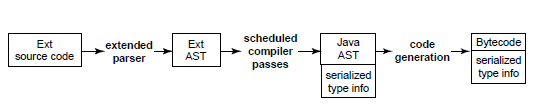
\includegraphics[width=0.8\textwidth]{polyglotarch.png}
\caption{Polyglot Architecture as per \cite{polyglotpaper}.}
\label{fig:polyglotarch}
\end{center}
\end{figure} 

As shown in \autoref{fig:polyglotarch} the first step in the creation of a new extension is to specify the syntax and generate a parser in order for the source code to be transformed into an Abstract Syntax Tree (AST) node structure. Polyglot comes with a parser generator, PPG, that allows the developer to implement the syntax extension based on additions or modifications of existing Java syntax rules\cite{polyglotpaper}.

Polyglot allows the user to define new AST nodes whose constructors can be called via the \textit{node factory} from the generated parser and additional information about the code structure can be encoded within these nodes. 

A \textit{type system} is also offered by the extension framework which acts as a factory for objects representing types and related constructs such as method or class signatures\cite{polyglotpaper}.

At the core of the compilation process lies the sequence of passes through the tree, which traverse all AST nodes and transform them as defined by the pass implementations. Some of these passes, i.e. the type checking pass, can halt the compilation process if the generated tree does not conform to the predefined rules. 

If the pass succeeds another AST tree is generated with the aim of finally generating a tree structures that is equivalent to a Java code tree. The resulting code is then passed to \LST{javac} which compiles is into byte code that can be executed on an Java Virtual Machine.

\subsection{Implementation}
\label{subsec:polyglotimpl}

The Polyglot Parser Generator (PPG) is implemented as a pre-processor for the CUP LALR parser generator\cite{cuplalr}. PPG uses a language-independent syntax definition style based on productions. The definitions are sequences of tokens, with the basic unit of specification being a \textit{terminal token}. Groups of tokens can be defined as \textit{non-terminal tokens} and non-terminal tokens can be grouped agin into other non-terminal tokens, faciliting definition reuse. When the syntax of an extension is specified, the programmer can extend, modify or delete some of the definitions form the given PPG as Polyglot supports grammar inheritance bewteen the default set and the extension. Examples of such language definitions can be found in \autoref{subsec:ppgimpl}.

The package \LST{polyglot.ast} contains the AST node classes used to represent the Abstract Syntax Tree. Polyglot implements all node classes for Java constructs, such as constructor calls, method calls, casts, synchronized methods, blocks and definitions. Each of the nodes inherits its main functionality from \LST{polyglot.ast.Node}.

As discussed, the actual compilation process is performed by a series of pases. The definitions of passes as well as their order is defined in an extension's ExtensionInfo class and the passes are executed in an order scheduled by the scheduler, which ensures that all dependencies between compilation units are satisfied. The most notable passes from the default set are \textit{parsing}, \textit{build-types}, \textit{disambiguate} and \textit{type checking} with all their respective implementations located in \LST{polyglot.visit}. The final \textit{translation} pass transforms each AST node to a String and writes it to a \LST{.java} output file to be compiled with the standard Java compiler.

		
%%%%%%%%%%%%%%%%%%%%%%%%%%%%%   SESSION JAVA   %%%%%%%%%%%%%%%%%%%%%%%%%%%%%%%%%%%%%%%
		
\section{Session Java (SJ): Implementing Binary Session Types}
\label{sec:sessionj}

	
Session-Based Distributed Programming as described in \cite{sessionbased_programming} integrates session-types discussed in \autoref{sec:binsessiontypes} and object-oriented programming in Java providing the programmer with a new tool to ensure soundness and correct execution of communications between distributed parties. The implementation of the runtime and compiler framework guarantees the desired properties both statically at compilation by checking whether the specified interactions match the declared protocol and dynamically through checking at runtime between the parties. The work from \cite{sessionbased_programming} is described in detail in the following sections.

\subsection{Programming in SJ}
\label{subsec:sjprogram}

Session programming consists of two steps: specifying the intended interaction protocol and implementing these protocols using session types.

Protocol specification can be clearly illustrated using the example of an ATM interacting with bank servers, in which the ATM submits a query with the user's id accompanied with the amount he/she would like to withdraw. If the amount is available, the bank returns true, else false is returned. This process can be iterated by the ATM as many times as needed for different amounts. If the customer confirms the withdrawal the ATM sends the amount again and the bank returns true if the transaction was completed successfully.

\begin{table}[H]
\center
\caption{Protocol Specification Code}
\begin{tabular}{|l|l|}
\hline

  \begin{lstlisting}[basicstyle=\LISTINGSTYLE]
  protocol query {
    begin.
    ![
        !<Double>.
        ?(Boolean)
    ]*.
    !{
      ACCEPT: !<Double>.
              ?(Boolean),
      REJECT:
    }
  }
  \end{lstlisting}
  &
  \begin{lstlisting}[basicstyle=\LISTINGSTYLE]
  protocol answer {
    begin.
    ?[
        ?(Double).
        !<Boolean>
    ]*.
    ?{
        ACCEPT: ?(Double).
                !<Boolean>,
        REJECT:
    }
  }
  \end{lstlisting}\\
  \hline
  
\end{tabular}
\label{CODEprotocol}
\end{table}

The code fragment shows how a protocol is specified, in particular sending a type is specified as \LST{!<Type>} and dual action of receiving as \LST{?(Type)}. Iterations are depicted by \LST{![...]*} for the controlling part and \LST{?[...]*} by the following part, where the * can be replaced with a fixed number of iterations. Finally, branching is specified by \LST{!\{LABEL1:..., LABEL2:...\}} for the controlling party and the dual identifier is \LST{?\{LABEL1:..., LABEL2:...\}}.

The next step is to establish a \textit{Session server socket} listening for session requests alongside a \textit{Session server address} specifying the socket's address and type of connection it accepts. Additionally, the \textit{socket} itself has to be created which represents the channel through which all communications are performed. The server-side code accepting connections therefore looks as follows:

\begin{lstlisting}%[basicstyle=\LISTINGSTYLE, numbers=left]
/* create SJServerSocket for incoming requests */
SJServerSocket bank_accept = SJServerSocketImpl.create(answer, 1452);

/* create SJSocket for accepting requests */
SJSocket bank_socket = null;

/* accept incoming request */
bank_socket = bank_accept.accept();
\end{lstlisting}

The client, in this case the ATM can request the service from the bank in the following way:

\begin{lstlisting}%[basicstyle=\LISTINGSTYLE, numbers=left]
/* create SJServerAddress at `host'*/
SJServerAddress atm_send =
        SJServerAddress.create(query, host, 1452);

/* create SJSocket for sending requests */
SJSocket atm_socket = SJSocketImpl.create(atm_send);

/* request a session with bank */
atm_socket.request();
\end{lstlisting}

\LST{SJSocket.send(Object)} and \LST{SJSocket.receive(Object)} methods can then be called on the instances of the sockets to send/receive data. Additionally the same methods are used for sending and receiving sessions, making the process very clear and concise.

Method \LST{SJSocket.outwhile(/*condition*/)} can be called on the controlling side of the iteration and \LST{SJSocket.inwhile()} on the receiving part to iteratively follow the sender.

Finally \LST{SJSocket.outbranch(ACCEPT)} can be called to select the desired branch. On the receiving end 
\LST{SJSocket.inbranch()\{case: ACCEPT \{..\} case:REJECT\{..\}} is called for branching off in the desired direction. The process of setting up the connection is as simple as the configuration of RMI or UDP connections, however added safety of execution is provided.



\subsection{SJ Framework Design}
\label{subsec:sjdesign}

The SJ Framwork is organised around the three following layers in which actions are taken depending on the session types currently processed. By going through each of the layers, the user code programmed transport-independtly in SJ is compiled into concrete communication actions based around a certain transport in Java.

\begin{packed_description}
\item[Layer 1] SJ source code.
\item[Layer 2] Java translation and session runtime APIs.
\item[Layer 3] Runtime execution: JVM and SJ libraries.
\end{packed_description}

The compiler maps Layer 1 onto Layer 2, resulting in type-checked Java code. During this process session-operations are checked against the specified protocol and translated into communication primitives supported by SJ Runtime. Layer 3 then executes the resulting code over concrete data transfer protocols and performs the dynamic type-checking in order to ensure runtime compliance of data exchange.

The authors envisage programmers to agree on a communication protocol and then code their sections of the code accordingly. This permits Layer 2 to check individual party's communications against the session-type, often referred to as protocol. The protocol is then also used to ensure that the two parties that engage in a session use the same protocol, i.e. that the same structure of the conversation is desired by both peers.


\subsection{SJ Compiler Design and Structure}
\label{subsec:sjcomp} 

\paragraph*{Compiler Design Principles}
The SJ compiler is based on the Polyglot extensible compiler framework (as discussed in \autoref{sec:polyglot}), which forms the foundation for compiling the standard Java syntax. The SJ compiler, as it inherits its basic functionality from Polyglot, is therefore capable of performing the type-checking against the requirements of both Java and the additional SJ rules. 

In the special compilation case of session types, the sockets are being validated for linear usage to prevent any concurrent usage. It is verified that each session implementation conforms to the protocol with regards to conversation structure and the types of messages exchanged. This is also true for session delegation where the accepted sessions in the methods are checked against the protocols.

Notably, the design of the session types is implemented according to object-orientation guidelines, implementing \textit{session subtyping}, an inheritance structure for these special types. This permits message type variance, for example receiving a subtype of the type specified in the protocol or structural subtyping for branching. In the latter case the deciding party of the branching structure may only wish to cover a set from the range of branches covered by the protocol, which is allowedd according the SJ structural subtyping principles.

\paragraph*{Compiler Implementation Details}
As briefly mentioned above the SJ Compiler follows the design principles of Polyglot. 

A range of additional AST nodes are introduced to represent the SJ syntax in form of an Abstract Syntax Tree (AST). This includes nodes for the protocol declarations, currently stored in form of local variable declarations or field declarations. Further on, there are nodes for all basic SJ operations, compound operation such as branching and recursion and nodes to support session delegation. Nodes have also been added to enable session channels and their creation. All nodes are created by  \LST{sessionj.ast.SJNodeFactory} serving as a node factory class from which the relevant constructors are called.

The package \LST{sessionj.parse} contains the extension to the Polyglot parser generator which specifies the necessary additions to the standard Java syntax. This includes syntactic rules for the specification of protocols and session operations together with any other definitions needed by the Polyglot framework.

The SJ type system is implemented in the packages within \LST{session.types} with classes that contain type information about SJ objects. The types in this package provide the foundation for the type-checking during compilation and runtime as they implement the \textit{session type theory} discussed in \autoref{sec:binsessiontypes}. As in the case of AST nodes, types are created through calls to relevant methods in the \LST{sessionj.types.SJTypeSystem} interface, where the type constructors are called from.

Finally, compilation process is coordinated by visitor passes in the order specified in \LST{sessionj.ExtensionInfo}. The SJ passes are responsible for building the types, parsing operations, performing the type checking and then translating the nodes into standard Java nodes for the code to be ready for compilation with the standard Java compiler. All the passes are implemented in the \LST{sessionj.visit} package and run when the \textit{sessionjc} compiler is invoked.


\subsection{SJ Runtime Design and Structure}
\label{subsec:sjrun}

\paragraph*{Runtime Design Principles}
The main responsibility of the runtime is to support all basic interaction methods through the underlying transfer protocols. This includes the basic and compound operations, and also the session delegations. Additionally, the SJ Runtime is designed to ensure dynamic validation of the interaction between the two parties. It was intended for the runtime to check session compatibility on session initiation by checking the received session type against the locally stored one. Further on the SJ Runtime also has the task of live session monitoring to ensure compliance of \textit{sends} and \textit{receives} against the types declared in the protocols. This prevents software from being validated correctly but suddenly adversely changing its behaviour. Finally, the runtime is also responsible for remote class loading, a feature similar to that of Java RMI. 

\begin{figure}[htb]
\begin{center}
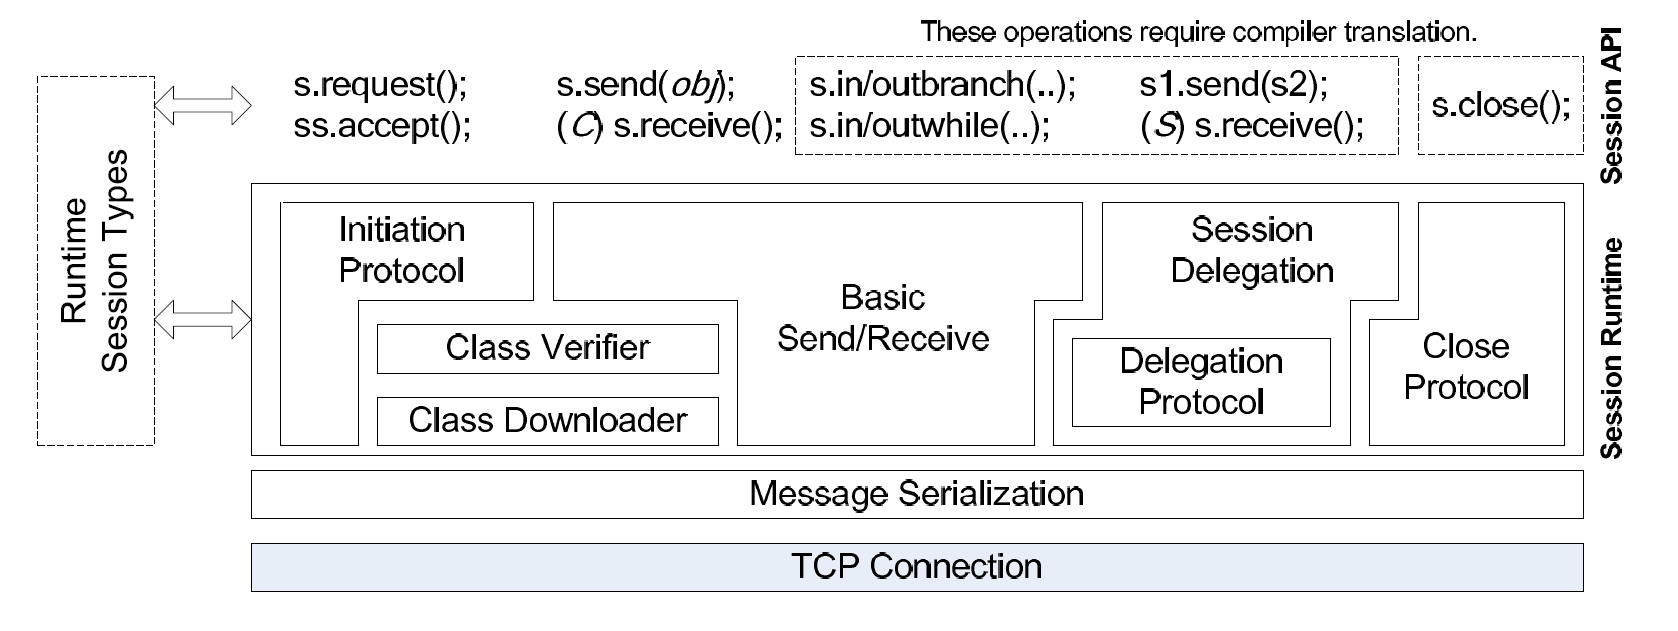
\includegraphics[width=0.8\textwidth]{sjruntime.png}
\caption{The structure of the SJ session runtime as per \cite{sessionbased_programming}.}
\label{fig:sjruntime}
\end{center}
\end{figure}

\paragraph*{Runtime Structure}
The structure of SJ Runtime, which is effectively a \LST{.jar} library file that every program written in SJ has to import is shown in \autoref{fig:sjruntime}.

The Session API, depicted as the upper-most layer facilitates the main operations that can be performed on a session, such as requesting, accepting and closing a session, as well as performing the sending, receiving and all compound session operations. It is worthwhile noting that some the operations specially marked in the Figure are translated into more complex SJ Runtime method calls by the compiler. This layer is the main and only point of interaction between the programmer and the underlying infrastructure.

The \textit{initiation protocol} is invoked when the \LST{request()} and \LST{accept()} methods are called. The connection over the underlying transport is then established and the session compatibility between the peers verified. This is enforced when the parties exchange the session types which they implement and each independtly checks compatibility. At this stage each of the parties can raise exceptions, which terminate the session in case there is a disagreement on the session types. The initiation protocol can also perform eager class downloading, in case a class definition is needed for one of the receieved types.

Once the interaction is underway, basic send and receive operations can be performed. Each such call invokes runtime monitoring actions across several classes to ensure that received types are equal to expected types. Basic operations also facilitate branching and looping cases, as a single branch case or loop condition value can be sent in form of a basic message. The messages, either as primitive types or objects are transmitted through the byte stream of the underlying transport, using standard Java serialization, as depicted in \autoref{fig:sjruntime}. Note that this figure shows the example of TCP, however currently UDP, HTTP and HTTPS are also supported.

The SJ Runtime implements a class loader, which can perform remote class loading enabling the communication of concrete message types that implement the abstract types of a protocol specification. Classes can be downloaded \textit{eagerly} (i.e. download all classes that may be needed at session initiation or \textit{lazily} (download just as needed) from an HTTP repository. Class verification can also be performed using the SerialVersionUID checks of all shared classes for equality.

Finally, the session is closed using the implicit \LST{close()} method. The method is called when both parties finish their parts of the conversation. Alternatively, the session can terminate when one of the session peers raises an exception, in which case \LST{close()} propagates the failure signal to both peers. The last case of session termination can arise due to asynchrony possible in cases of session delegation.


	

	
%%%%%%%%%%%%%%%%%%%%%%%%%%%%%%%%%%%%%%%%%%%%%%%%%%%%%%%%%%%%%%%%%%%%%%%%%%%%%%%%%%%%%%%
% - BACKGROUND: END
%%%%%%%%%%%%%%%%%%%%%%%%%%%%%%%%%%%%%%%%%%%%%%%%%%%%%%%%%%%%%%%%%%%%%%%%%%%%%%%%%%%%%%%


